\documentclass{patmorin}
\usepackage{amsmath,amsthm,graphicx}
\listfiles
\usepackage[mathlines]{lineno}
\linenumbers
\usepackage{pat}

\newtheorem{cor}{Corollary}
\DeclareMathOperator{\range}{range}

\title{Maximum Interference for Transmitters Uniformly Distributed on a Segment}
\author{Evangelos Kranakis, Danny Krizanc, and Pat Morin}

\begin{document}
\maketitle

\begin{abstract}
We consider the following problem: A set of $n$ transmitters are
place independently and uniformly at random on a unit interval.  Each
transmitter, except the two extreme ones, adjust their transmission ranges
so that they can be heard by the further of their left neighbour and right
neighbour.  What is the maximum number of transmitters that can be heard
by any individual transmitter?  We show that, with high probability,
there exists some transmitter that hears $\Omega(\sqrt{\log n})$
transmitters and all transmitters hear $O(\sqrt{\log n})$ transmitters.
\end{abstract}

\section{Introduction}

We consider the following problem: A set of $n$ transmitters are
place independently and uniformly at random on a unit interval.  Each
transmitter, except the two extreme ones, adjust their transmission ranges
so that they can be heard by the further of their left neighbour and right
neighbour.  What is the maximum number of transmitters that can be heard
by any individual transmitter? 

More formally, let $S=\{x_1,\ldots,x_n\}$ be a set of values chosen
independently and uniformly at random from the real interval $[0,1]$
and reordered so that $x_1<\cdots<x_n$.  For each $i\in\{2,\ldots,n-1\}$,
define the \emph{broadcast range}
\[
   R_i = \max\{x_i - x_{i-1}, x_{i+1}-x_i\}
\]
and the \emph{broadcast interval}
\[
   I_i = [x_i-R_i,x_i+R_i] \enspace .
\]
The \emph{interference at $x\in\R$} is then given by
\[
   Z(x) = |\{x_j\in S\setminus\{x\}: x \in I_j\}| \enspace .
\]
The \emph{maximum interference} in $S$, is given by
\[
   Z(S)=\max\{Z(x_i):i\in\{1,\ldots,n\}\} \enspace .
\]
We prove the following result:

\begin{thm}
With probability $1-o(1)$, $Z(S)\in \Theta(\sqrt{\log n})$.
\end{thm}

This result is an immediate consequence of \lemref{lower-bound} and
\lemref{upper-bound} which are proven in the next section.

\section{The Proof}

In this section we prove our main result, namely that the maximum
interference is $\Theta(\sqrt{\log n})$ with high probability.
Throughout this section, we will make use of the relationship between
uniformly distributed point sets and exponential random variables
\cite[Chapter~V, Theorem~2.2]{d86}.  Suppose $S$ is a set of $n$ points
independently and uniformly distributed in $[0,1]$ whose elements are
$x_1,\ldots,x_n$ in sorted order.  Let $X_0,\ldots,X_n$ be Exponential(1)
random variables, let $x'_i=\sum_{j=0}^{i-1}X_j$, and let $x_i''=x_i/x_{n+1}$.
Then $x_1'',\ldots,x_n''$ have the same distribution as $x_1,\ldots,x_n$.

Because of the above relationship we will, throughout this section, use
the convention that $X_0,\ldots,X_n$ are Exponential(1) random variables,
$x_i=\sum_{j=0}^{i-1}X_j$, and $S=\{x_1,\ldots,x_n\}$.  This definition
of $S$, $x_1,\ldots,x_n$, and $X_0,\ldots,X_n$ will be implicit in the
statements of all subsequent results and in all proofs.

\subsection{The Lower Bound}

We prove our lower-bound by by defining a configuration of points that
leads to an element with interference $\Omega(\sqrt{\log n})$ and then
showing that, with high probability, this configuration occurs somewhere
in our point set.

A sequence of numbers $X_0,\ldots,X_k$ forms a \emph{$k$-frame} if
\[
     1 \le X_0 \le 2
\]
and
\[
     X_{i-1}/4 \le X_i \le X_{i-1}/2 \enspace ,
\]
for all $i\in\{1,\ldots,k\}$.  Notice that, if $X_0,\ldots,X_k$ form a
$k$-frame, then $x_{k+1}$ is a node that has interference at least $k$.
The next lemma shows that this situation is not too unlikely:

\begin{lem}\lemlabel{frame}
If $X_0,\ldots,X_k$ are a sequence of independent Exponential(1) random
variables, then the probability that $X_0,\ldots,X_k$ form a $k$-frame
is at least $e^{-1}(1-e^{-1})2^{-(k+1)^2}$.
\end{lem}

\begin{proof}
Recall that an Exponential(1) random variable $X$ has cumulative
distribution function
\[
   \Pr\{X \le x\} = 1-e^{-x} \enspace .
\]
Next, observe that, in a frame,
\[
                 4^{-i} \le X_i \le 2^{-i}  \enspace ,
\]
for all $i\in\{0,\ldots,k\}$.  Let $F(X)$ be the event ``$X$ is a frame.''
Then,
\begin{align*}
     \Pr\{F(X_0,\ldots,X_{i+1}) \mid F(X_0,\ldots,X_{i})\} 
        & = \Pr\{X_{i+1} \in [X_{i}/4,X_{i}/2] \mid F(X_0,\ldots,X_{i})\} \\
        & \ge \Pr\{X_{i+1} \in [4^{-i}/4,4^{-i}/2]\} \\
        & = \Pr\{X_{i+1} \in [2^{-(2i+2)},2^{-(2i+1)}]\} \\
        & = \exp(-2^{-(2i+2)}) - \exp(2^{-(2i+1)}) \\
        & \ge 2^{-(2i+3)} \enspace ,
\end{align*}
where the last inequality holds for all $i\ge 0$.  Therefore,
\begin{align*}
     \Pr\{F(X_0,\ldots,X_{k})\}
   & = \Pr\{X_0\in[1,2]\}
         \cdot\prod_{i=1}^k \Pr\{F(X_0,\ldots,X_{i})
                                 \mid F(X_0,\ldots,X_{i-1})\} \\
   & = e^{-1}(1-e^{-1})
         \cdot\prod_{i=1}^k \Pr\{F(X_0,\ldots,X_{i})
                                 \mid F(X_0,\ldots,X_{i-1})\} \\
   & = e^{-1}(1-e^{-1})
         \cdot\prod_{i=1}^k \Pr\{X_{i} \in [X_{i-1}/4,X_{i-1}/2]\}
                                 \mid F(X_0,\ldots,X_{i-1})\} \\
   & \ge e^{-1}(1-e^{-1})
         \cdot\prod_{i=1}^k \Pr\{X_{i} \in [4^{-i}/4,4^{-i}/2]\} \\
   & \ge e^{-1}(1-e^{-1})\cdot\prod_{i=1}^k 2^{-(2i+1)} \\
   & = e^{-1}(1-e^{-1})\cdot2^{-\sum_{i=1}^k(2i+1)} \\
   & = e^{-1}(1-e^{-1})\cdot2^{-(k^2+2k)} \\
   & \ge e^{-1}(1-e^{-1})\cdot2^{-(k+1)^2} \\
\end{align*}
as required.
\end{proof}


\begin{lem}[Lower Bound]\lemlabel{lower-bound}
With probability at least $1-\exp(-n^{1-c}/\sqrt{c\log n})$, there exists
some element of $S$ that has interference at least $\lfloor\sqrt{c\log
n}\rfloor-2$.
\end{lem}

\begin{proof}
Let $k=\lfloor \sqrt{c\log n} \rfloor-1$.  By \lemref{frame},
$X_{jk},\ldots,X_{jk+k}$ have probability at least $2^{-(k+1)^2}\ge
n^{-c}$ of forming a $k$-frame, in which case $x_{jk+k}$ has
interference at least $k$.  Since this is true, independently, for any
$j\in\{0,\ldots,\lfloor n/k\rfloor\}$, the probability that there is no
element of $S$ with with interference greater than $k$ is at most
\[
   (1-n^{-c})^{\lfloor n/k\rfloor} \le \exp(-\lfloor n^{1-c}/k\rfloor) \enspace ,
\]
as required.
\end{proof}


\subsection{The Upper Bound}

We begin our upper-bound proof by studying a variant of interference that
is 1-sided and that considers only interference generated by transmitters
that are nearby.  The \emph{left-interference} of an element $x_t\in
S$ is the number of elements $x_i\in S$ such that $x_i < x_t$ and
$x_t-x_i \le \max\{x_i-x_{i-1},x_{i+1}-x_i\}$.  The \emph{short-range
left-interference} of $x_t$ is defined in the same way, except only
counting those elements $x_i$ such that $X_{i-1} \le 1$. (Note that this
implies $x_t-x_i \le 1$.)

\begin{lem}\lemlabel{squeaker}
The maximum short-range left-interference of any element in $S$ is at
most $\sqrt{c\log n}$ with probability at least $1-n^{-\Omega(c)}$.
\end{lem}

\begin{proof}
We will actually prove something stronger, namely that the short-range
left-interference of any point $x\in\R$ is at most $\sqrt{c\log n}$
with probability at least $1-n^{-\Omega(c)}$.  We first observe that the
maximum value of the short range interference occurs when $x$ is of the
form $x_{i} + X_{i-1}$, for some $i\in\{1,\ldots,n\}$ where $X_{i-1}
\le 1$.

Consider the following process, that begins with $X_0$ and
upper-bounds the short-range left-interference at $x=x_1+X_0=2X_0$
(see \figref{upper-bound}). If $X_0>1$, the process immediately ends.
Otherwise, the process proceeds in rounds where, in round $i$, there
is a length $\ell_i$.  Initially $\ell_i=X_0$.  During round~$i$, we
generate $X_{r_{i-1}+1},\ldots,X_{r_i}$ until $\sum_{j=1}^r X_{r_{i-1}+j}
\ge \ell_i/2$.  If $\sum_{j=1}^r X_j \ge \ell_i$, then the process ends.
Otherwise, we set $\ell_{i+1} = \ell_i-\sum_{j=1}^{r_i} X_j$ and continue
onto round $i+1$.

\begin{figure}
  \begin{center}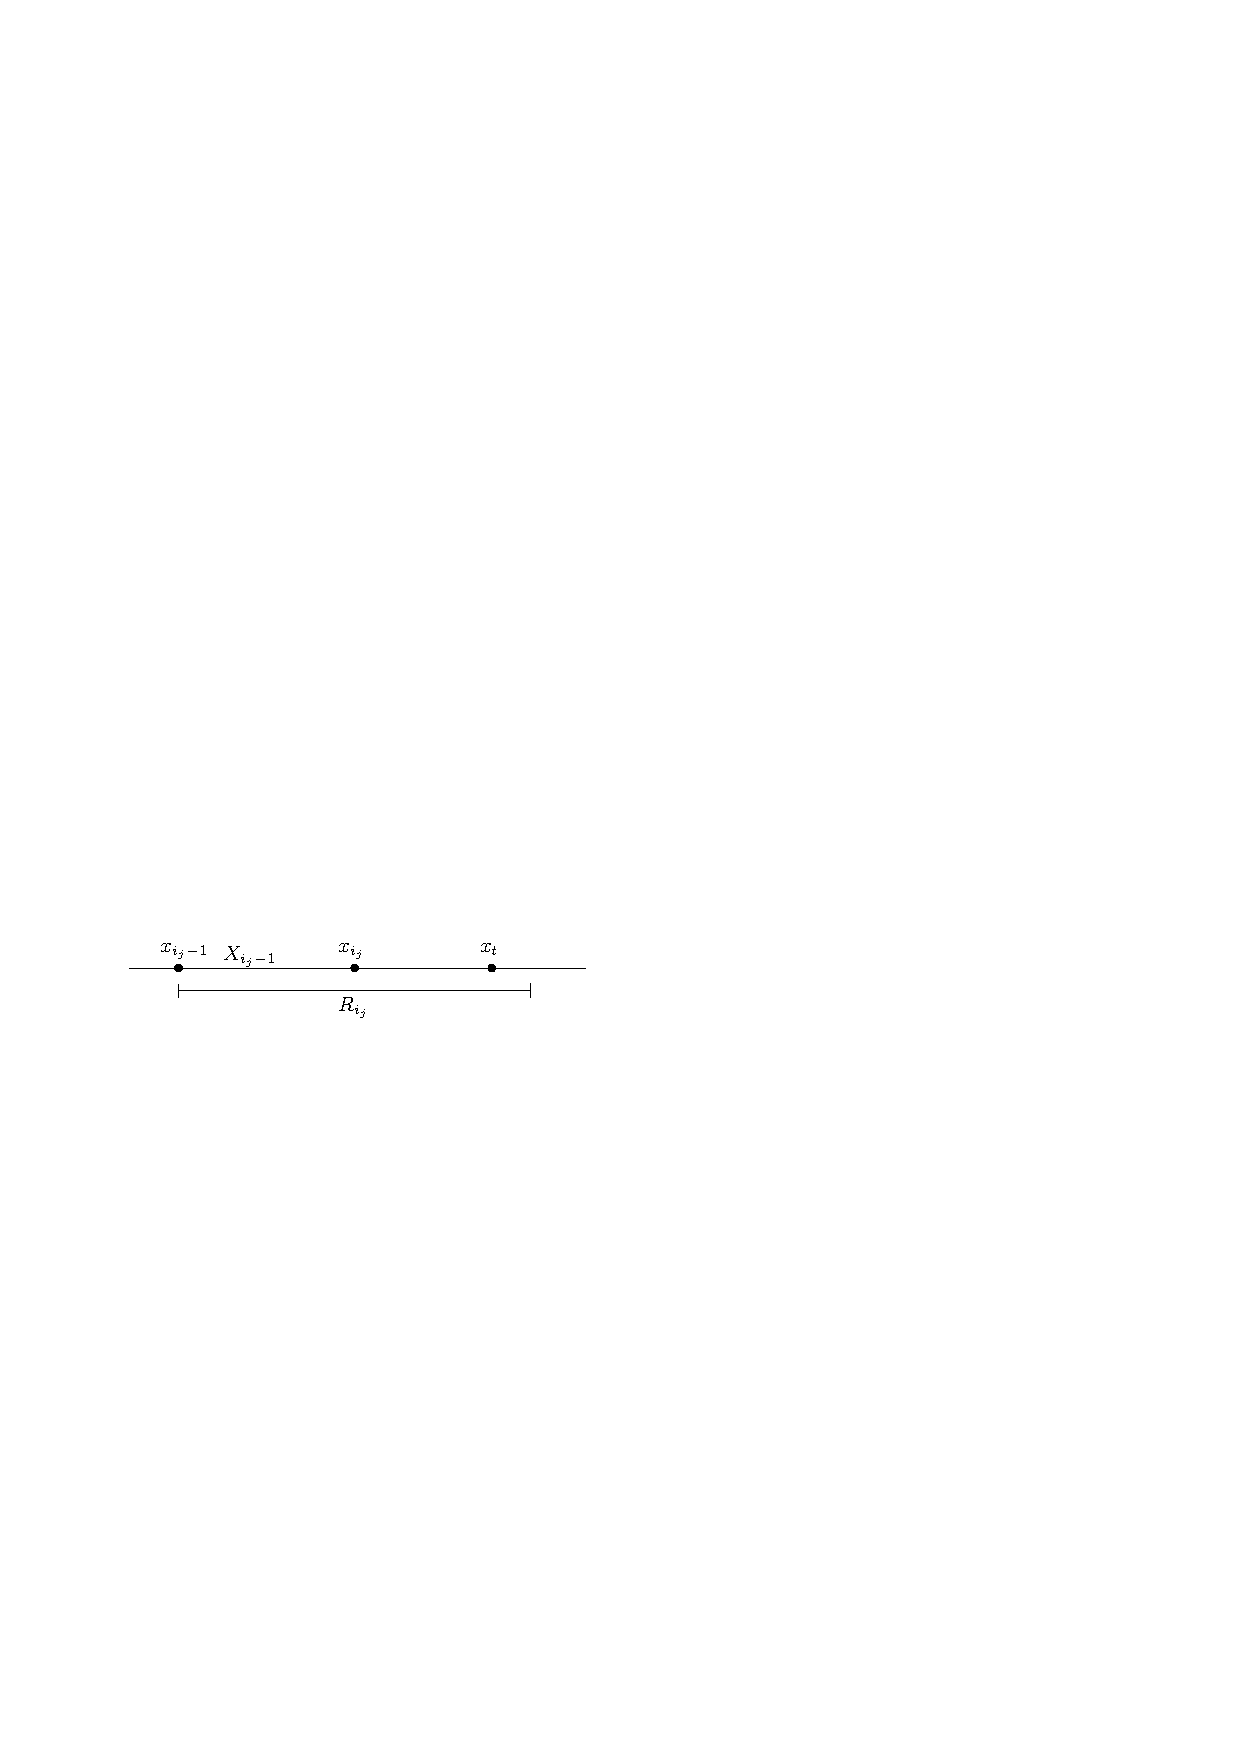
\includegraphics{upper-bound}\end{center}
  \caption{A process that leads to an interference of 3 at $x$.  The process ends because $X_4 > \ell_3$}
  \figlabel{upper-bound}
\end{figure}

Notice that, in this process, the only elements that might contribute
to the short-range left-interference at $x$ are $x_1$ and those $x_i$
where $X_{i-1}$ completes a round other than the final round.  Thus,
if the above process terminates during round $k$, then the short-range
left-interference at $x$ is at most $k$.

Now, observe that in round $i$, $\ell_i \le 1/2^{i-1}$.  Therefore,
the probability of continuing to round $i+1$ from round $i$ is at most
\[
   \Pr\{X_{r_{i-1}+1} \le 1/2^{i-1}\} = 1-e^{-2^{-i+1}} \le 2^{-i+1} \enspace .
\]
Therefore, the probability of continuing up to round $k$ is at most
\[
  \prod_{i=1}^{k-1} 2^{-i+1}
  = 2^{-\sum_{i=1}^{k-1}(i+1)}
  = 2^{-(k+2)(k-1)/2} \le 2^{-k^2/2} \enspace ,
\]
for $k\ge 2$.  Taking $k=\sqrt{c\log n}$, we find that this probability
is at most $1/n^{c/\sqrt{2}}$.  Therefore, the probability that there
is \emph{any} point $x\in\R$ with short-range left-interference greater
than $\sqrt{c\log n}$ is at most $1/n^{c/\sqrt{2}-1}$, as required.
\end{proof}


Finally, we have all the pieces needed to complete the upper bound

\begin{lem}[Upper Bound]\lemlabel{upper-bound}
With probability at least $1-n^{-\Omega(c)}$, the maximum interference of
any element in $S$ is at most $\sqrt{c\log n}$.
\end{lem}

\begin{proof}
We consider only left-interference, since the right-interference
can be bounded in a symmetric way.  Consider some element $x_t$.  The
left-interference of $x_t$ is generated by some elements
$x_{i_0},\ldots,x_{i_k}$ where $x_{i_k}<\cdots<
x_{i_0}<x_t$.  \lemref{squeaker} already bounds the number of elements of this
sequence where $X_{i_j-1} \le 1$.  Thus, all that remains is to bound
the number of elements $x_{i_j}$ where $X_{i_j} > 1$.

Observe, as in the proof of \lemref{squeaker}, that, for any
$j\in\{1,\ldots,k\}$, in order for $x_{i_j}$ to interfere with $x_t$
we must have
\[
   X_{i_j-1} \ge x_t - x_{i_j}
\enspace ,
\]
which implies that $X_{i_j-1} \ge 2 X_{i_{j-1}-1}$ for all
$j\in\{1,\ldots,k\}$.  Therefore, if we have $2^r$ elements with
$X_{i_j}>1$, then we have some element $X_{i_k-1} > 2^r$.  The probability
that a particular $X_i$ is greater than $2^r$ is $e^{-2^r}$. Therefore,
the probability that there exists any $X_i$ greater than $2^r$ is at most
$ne^{-2^r}$.  Setting $r=d\log\ln n$ for a sufficiently large constant
$d>1$ makes this probability at most $n^{1-d}$, and completes the proof.
\end{proof}

\bibliographystyle{plain}
\bibliography{interference}



\end{document}

